% $Id: template.tex 11 2007-04-03 22:25:53Z jpeltier $

%\documentclass{vgtc}                          % final (conference style)
\documentclass[review]{vgtc}                 % review
%\documentclass[widereview]{vgtc}             % wide-spaced review
%\documentclass[preprint]{vgtc}               % preprint
%\documentclass[electronic]{vgtc}             % electronic version

%% Uncomment one of the lines above depending on where your paper is
%% in the conference process. ``review'' and ``widereview'' are for review
%% submission, ``preprint'' is for pre-publication, and the final version
%% doesn't use a specific qualifier. Further, ``electronic'' includes
%% hyperreferences for more convenient online viewing.

%% Please use one of the ``review'' options in combination with the
%% assigned online id (see below) ONLY if your paper uses a double blind
%% review process. Some conferences, like IEEE Vis and InfoVis, have NOT
%% in the past.

%% Figures should be in CMYK or Grey scale format, otherwise, colour 
%% shifting may occur during the printing process.

%% These three lines bring in essential packages: ``mathptmx'' for Type 1 
%% typefaces, ``graphicx'' for inclusion of EPS figures. and ``times''
%% for proper handling of the times font family.

\usepackage{mathptmx}
\usepackage{graphicx}
\usepackage{times}
\usepackage{mathtools}
\usepackage[capitalise, noabbrev]{cleveref}
\usepackage[usenames]{color}
\usepackage{textcomp}
\usepackage{gensymb}
\usepackage[detect-all]{siunitx}

\usepackage{libertine} 
\usepackage{siunitx}
\sisetup{per-mode=symbol,per-symbol = p}
%\sisetup{detect-all}
%\DeclareSIUnit{\sample}{S}
%% We encourage the use of mathptmx for consistent usage of times font
%% throughout the proceedings. However, if you encounter conflicts
%% with other math-related packages, you may want to disable it.

%% If you are submitting a paper to a conference for review with a double
%% blind reviewing process, please replace the value ``0'' below with your
%% OnlineID. Otherwise, you may safely leave it at ``0''.
\onlineid{112}

%% declare the category of your paper, only shown in review mode
\vgtccategory{Research}

%% allow for this line if you want the electronic option to work properly
\vgtcinsertpkg

%% In preprint mode you may define your own headline.
%\preprinttext{To appear in an IEEE VGTC sponsored conference.}

\newcommand{\todo}[1]{\textcolor{red}{\textbf{#1}}}

\title{A Lightweight H.264-based Hardware Accelerated Image Compression Library}

%% This is how authors are specified in the conference style

%% Author and Affiliation (single author).
%%\author{Roy G. Biv\thanks{e-mail: roy.g.biv@aol.com}}
%%\affiliation{\scriptsize Allied Widgets Research}

%% Author and Affiliation (multiple authors with single affiliations).
%%\author{Roy G. Biv\thanks{e-mail: roy.g.biv@aol.com} %
%%\and Ed Grimley\thanks{e-mail:ed.grimley@aol.com} %
%%\and Martha Stewart\thanks{e-mail:martha.stewart@marthastewart.com}}
%%\affiliation{\scriptsize Martha Stewart Enterprises \\ Microsoft Research}

%% Author and Affiliation (multiple authors with multiple affiliations)
%%\author{Roy G. Biv\thanks{e-mail: roy.g.biv@aol.com}\\ %
%%        \scriptsize Starbucks Research %
%%\and Ed Grimley\thanks{e-mail:ed.grimley@aol.com}\\ %
%%     \scriptsize Grimley Widgets, Inc. %
%%\and Martha Stewart\thanks{e-mail:martha.stewart@marthastewart.com}\\ %
%%     \parbox{1.4in}{\scriptsize \centering Martha Stewart Enterprises \\ Microsoft Research}}
\author{Jie Jiang \thanks{e-mail: jjiang24@uic.edu}\\ %
        \scriptsize University of Illinois at Chicago %
\and Thomas Fogal\thanks{e-mail: tfogal@nvidia.com}\\ %
     \scriptsize NVIDIA %
\and Cliff Woolley\thanks{e-mail: jwoolley@nvidia.com}\\ %
     \scriptsize NVIDIA %
\and Peter Messmer\thanks{e-mail: pmessmer@nvidia.com}\\ %
     \scriptsize NVIDIA} %


%% A teaser figure can be included as follows, but is not recommended since
%% the space is now taken up by a full width abstract.
%\teaser{
%  \includegraphics[width=1.5in]{sample.eps}
%  \caption{Lookit! Lookit!}
%}

%% Abstract section.
\abstract{
Hardware video encoding can lower the perceived latency for remote
visualization. We have created a lightweight library that simplifies
the use of NVIDIA's video compression hardware. We achieve overall
latencies below 15ms with compression ratios of approximately 140:1. To
verify its applicability in real world scenarios, we integrated our library
into ParaView. This offloads the encoding within ParaView to the GPU
and provides a 42x bandwidth reduction compared to existing image compression.}

%% ACM Computing Classification System (CCS). 
%% See <http://www.acm.org/class/1998/> for details.
%% The ``\CCScat'' command takes four arguments.

%\CCScatlist{ 
%  \CCScat{K.6.1}{Management of Computing and Information Systems}%
%{Project and People Management}{Life Cycle};
%  \CCScat{K.7.m}{The Computing Profession}{Miscellaneous}{Ethics}
%}

%% Copyright space is enabled by default as required by guidelines.
%% It is disabled by the 'review' option or via the following command:
% \nocopyrightspace

%%%%%%%%%%%%%%%%%%%%%%%%%%%%%%%%%%%%%%%%%%%%%%%%%%%%%%%%%%%%%%%%
%%%%%%%%%%%%%%%%%%%%%% START OF THE PAPER %%%%%%%%%%%%%%%%%%%%%%
%%%%%%%%%%%%%%%%%%%%%%%%%%%%%%%%%%%%%%%%%%%%%%%%%%%%%%%%%%%%%%%%%

\begin{document}

%% The ``\maketitle'' command must be the first command after the
%% ``\begin{document}'' command. It prepares and prints the title block.

%% the only exception to this rule is the \firstsection command
\firstsection{Introduction}

\maketitle

Image compression is commonly used in remote visualization systems to
create a smoother user experience over low-bandwidth links. Current
systems generally consider each image in isolation even though image
differencing approaches can yield considerable data savings.

H.264 is a block-oriented motion-compensation-based video compression
standard~\cite{wiegand2003overview}. The standard provides high
compression ratios but this ability comes at significant computational
expense.  Modern NVIDIA hardware provides a hardware-accelerate H.264
encoder~\cite{nvcodec}.  The hardware enables real-time encoding with
minimal overhead. Support for the encoder has been
integrated into popular multimedia frameworks~\cite{ffmpeg}.

\section{Design}

Our library can utilize NVIDIA's hardware encoder or the libx264-based
software encoder. We specifically designed our library to abstract away
most video compression configuration. A detailed discussion of
H.264 parameters is covered in~\cite{wiegand2003overview}. We have configured
the encoder to use settings reasonable for visualization. For example, video
compression normally has a lag time on the order of tens of frames. We have
reduced the lag time to a single frame and guaranteed that the encoder produces
a single buffer for every input image, which matches how tools such as 
ParaView~\cite{henderson2004paraview} and VisIt use image compressors today.

Our library handles only image compression and decompression. It leaves the
network communication to the user for ease of integration.

%NvPipe is built on top of FFmpeg to provide compatibility across systems with and without H.264 hardware. 
%Although NvPipe accepts images with format RGB/RGBA/YUV, it will convert the image into NV12 to before passing it to FFmpeg/NVENC. As is the decompressed image.

\subsection{Performance}

We measured three aspects of our compression libraries performance:
computational efficiency, compression ratio, and image quality.

\subsubsection{Compression Ratio}

%put the reference here: http://www.adobe.com/content/dam/Adobe/en/devnet/video/articles/h264_primer/h264_primer.pdf

% is there an actual argument for the bitrate?

Compression ratio is determined by the average bitrate parameter.
A guideline for bitrate setting is the Kush
Gauge~\cite{iszaidyinvestigation}:

\begin{equation}
\label{eq:bitrate}
 bitrate = resolution * \text{framerate} * f_m * 0.07 
\end{equation}

Where \(f_m\) is the `motion factor' that defines the estimated motion
of the video on a scale from 1 to 4, with 1 indicating the least motion
and 4 the most. The default bitrate used in the library uses 
\(f_m=4\) and an estimated 24 frames per second.

The compression ratio \(r_c\) for an 8-bit RGB image is calculated
using~\cref{eq:compress_ratio}.

\begin{multline}
\label{eq:compress_ratio}
 %\text{Compression\, ratio:} \\
 r_c = \frac{ resolution * \text{framerate} * 3 * 8}{ bitrate} = \frac{3*8}{0.07f_m} = \frac{343}{f_m} : 1
\end{multline}

\subsubsection{Image Fidelity}

Our library utilizes encoder settings for the lossy variant of H.264. Though
these settings can introduce artifacts at sharp edges in the image,
~\cref{fig:quality} demonstrates that these artifacts are minor.

\begin{figure}[h]
  \centering
  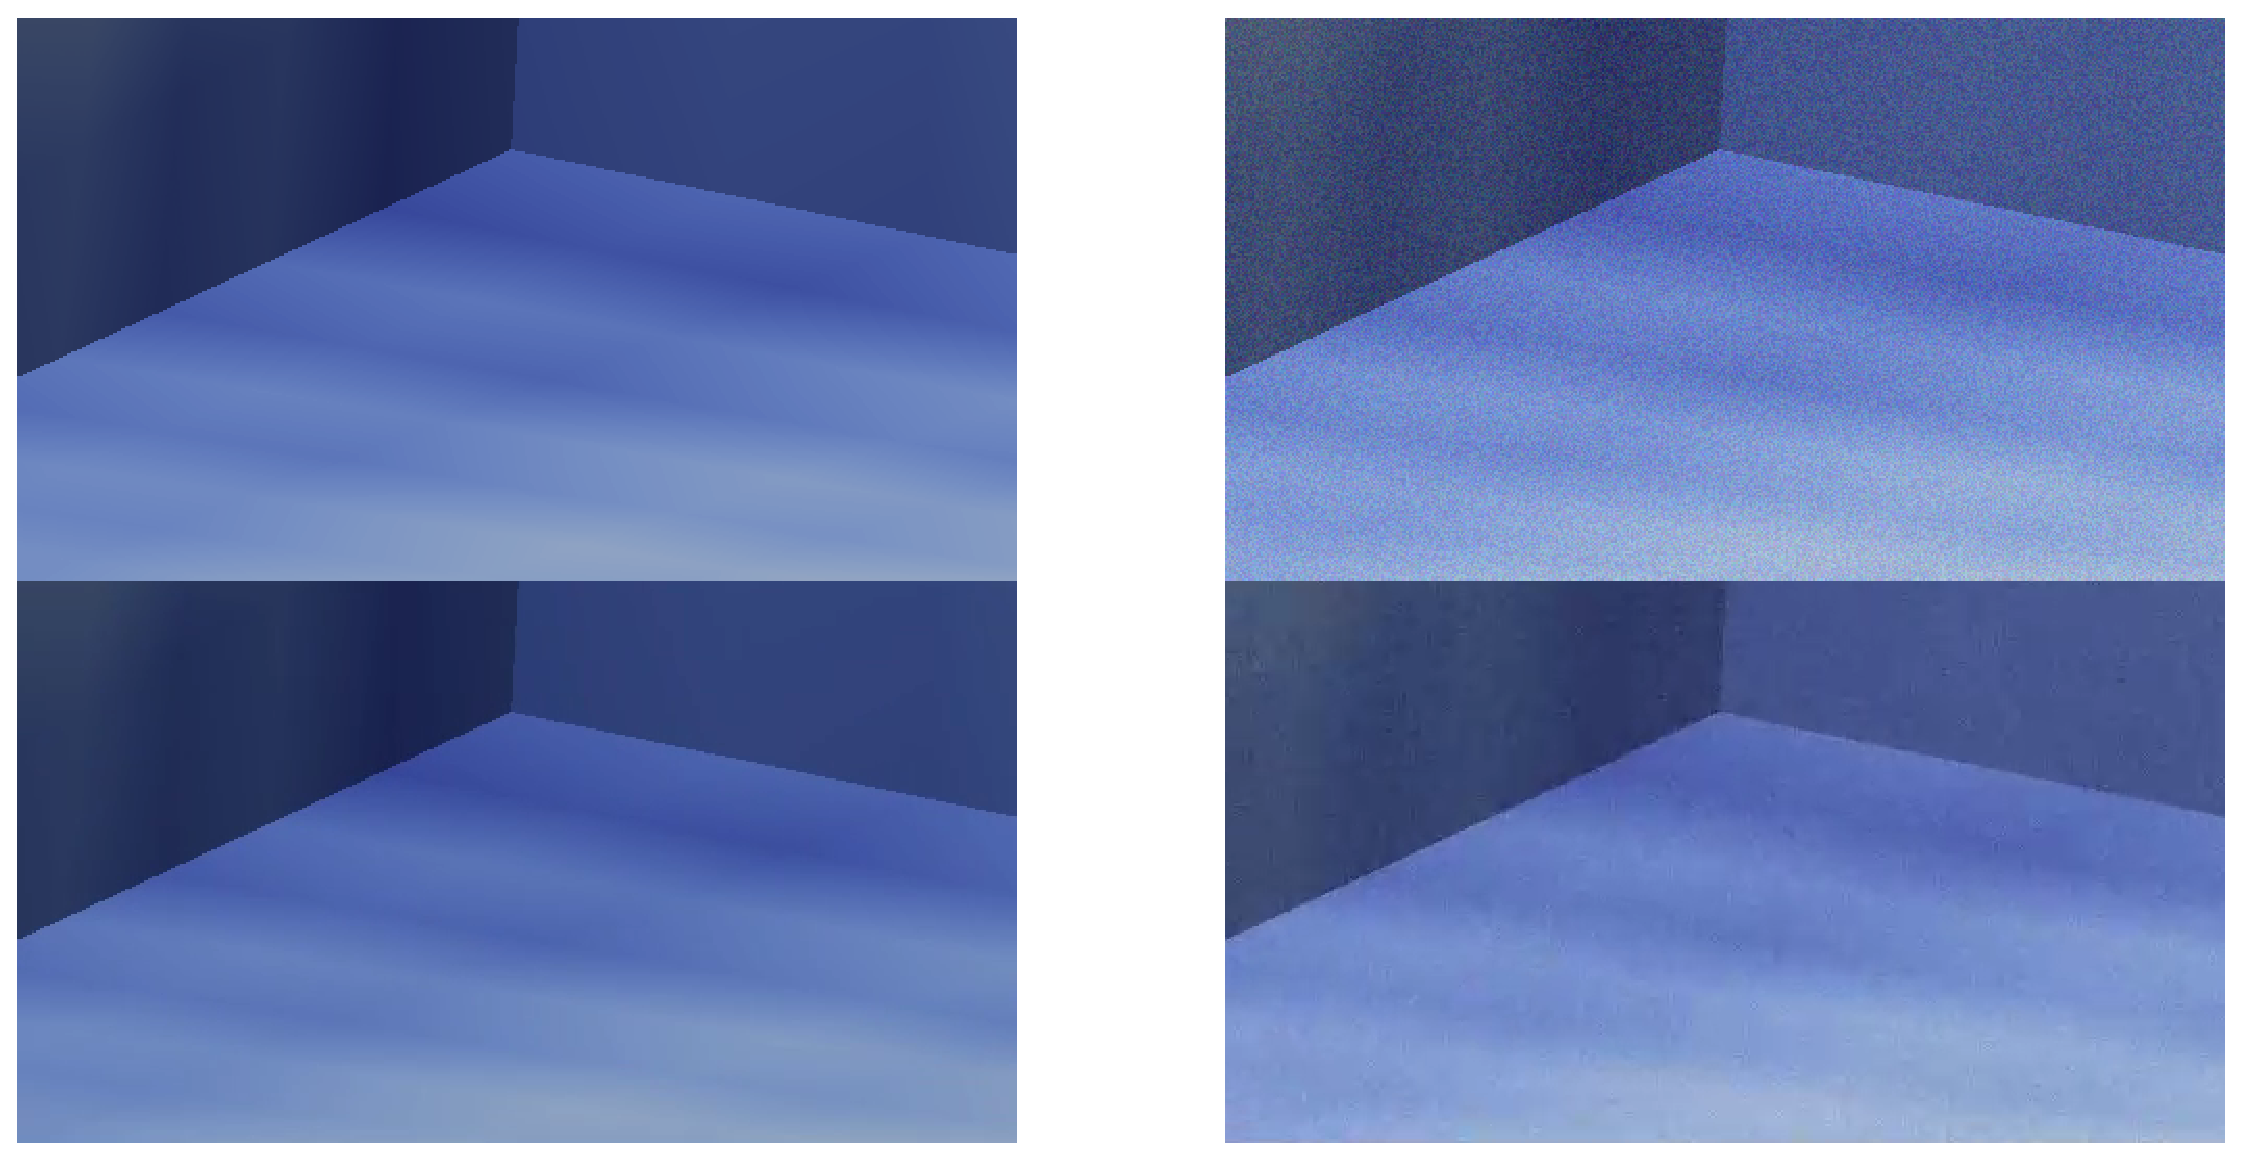
\includegraphics[width=\columnwidth]{quality.eps}
  \caption{1080p image compressed using bitrate calculated with
  \(f_m=4\). The image on the left is the original and the image on the right
  is the recovered. Average structural similarity (SSIM~\cite{wang2004image})
  between the images is 98\%.}
  \label{fig:quality}
\end{figure}

\section{Results}

%Our experiment setup contains two parts. In part one we benchmark the performance of our library given different resolutions and bitrates. In part two we implement vtkNvpipeCompressor to integrate NvPipe into Paraview. We create a distribute visualization use case and compared the performance of NvPipe with ParaView's native built-in compressor.

We performed a number of experiments to evaluate the utility of H.264
for visualization. All tests were run on an Ubuntu 16.04 machine with a
NVIDIA GeForce GTX 1080 (Pascal) graphics card.

%Both input and output buffer for compression and decompression are located on host memories. 

Ideally one would source the input images from the already-rendered
images on the GPU. However, existing remoter visualization systems are
not architected to easily adhere to this design (compositing often uses
images in host memory). Therefore we utilize an interface that accepts
data from host memory instead of GPU memory.

We ran a number of benchmarks to examine the performance and
compression ratio of our library. We tested a variety of resolutions to
elucidate the relationship between the codec's performance.  We also
tried a variety of bitrates but do not highlight the result here
because the results are what one might expect: lower bitrates compress
to smaller payloads.

%We set up experiment groups using 4 common resolutions. For each
%one we run 3 cases with low bitrate, medium bitrate and high bitrate
%settings. The medium setting uses~\cref{eq:bitrate} with \(f_m =1\)
%to calculate the bitrate. While low and high uses \(f_m\) of 0.5
%and 2 respectively. Each case runs 300 cycles of compressing and
%decompressing of consecutive images generated with moving color
%pattern.

Secondly, we integrated our library into ParaView and compared its
performance with and without hardware acceleration to
built-in compressors utilizing lz4, squirt and Zlib. Our library used a high
bitrate setting where \(f_m=4\) for best image quality. The existing
ParaView compressors were configured for maximum compression as opposed
to maximum performance, though we found little performance difference
between the two extremes.  The experiments used 1080p RGBA images (the
library removes the alpha channel) generated from a rotating volume
dataset.  We tried both a `high coherency' mode, rotating by
$1.2\degree{}$ per frame to roughly approximate interactive ParaView
use, and a `low coherency' mode that utilized a larger $45\degree{}$
rotation between
images, corresponding to a more extreme \textit{in situ} case.  Results
are the average from 300 iterations across five runs.

%Lz4 uses quality level 0. Squirt
%uses compression level 5. Zlib uses compression level of 9 for slow
%compression with highest compression ratio, color space reduction level
%of 5 and alpha channel stripping. Zlib fast uses compression level
%of 1 for fast compression with lowest compression ratio while other
%parameters remain the same. The experiments uses 1080p RGBA images
%generated from rotating volume dataset. The high coherency case applies
%a fixed small rotation angle of \(1.2\degree\) to the volume data per
%frame. The low coherency uses larger rotation angle of \(45\degree\)
%per frame. For each case we run 5 full test each with 300 cycles.

\subsection{Benchmark}
% library benchmark

% wouldn't mentioning linear regression make it easier to say this?

Our experimental data shows that the computational complexity is
linear with respect to the total number of pixels.  Furthermore, the
compression time is independent of the image contents.
~\cref{tab:experiment_setup} details bandwidth requirements and
performance for common resolutions.

%The benchmark experiment shows linear scalability of NvPipe to
%image size. Given the total number of million pixels of the image
%to be \(n_p\) and motion factor used for bitrate calculation to be
%\(f_m\). Linear regression analysis of compression time \(t_c\)
%and decompression time \(t_d\) generates the following models:
%\(t_c=2.27n_p+0.16f_m+0.86\) and \(t_d=1.60n_p+0.02f_m+0.89\) with
%\(R^2_c=99.92\%\) and \(R^2_d=99.97\%\). Performance is linear to total
%number of pixels in the image with trivial influence from the bitrate
%multipliccation factor used.

%%%%%%%%%%%%%%%%%%%%%%%%%%%%%%%%%
%   discuss it if extra room appears later.
%
%Each image compression or decompression call to NvPipe consists of
%format conversion and encoding or decoding API calls. Computational
%complexity for both tasks are linear to the totally number of pixels of
%the input or output image. So we could expect the overall complexity
%of our compression and decompression call remains linear to the image
%size.

\begin{table}[h]
  \caption{Average compression and decompression time per frame
  using our library.  Performance is essentially linear with
  respect to the size of the image.}
  \label{tab:experiment_setup}
  \scriptsize
  \begin{center}
    \begin{tabular}{cccc}
      Resolution & Bitrate(mbps) & Compress(ms) & Decompress(ms)\\
    \hline
      1024x768 & 1.651 & 2.8057 & 2.1170\\
      1280x720 & 1.935 & 3.4793 & 2.4304\\
      1920x1080 & 4.355 & 5.4358 & 4.2876\\
      4096x2160 & 18.579 & 21.2504 & 15.0976
    \end{tabular}
  \end{center}
\end{table}

\subsection{ParaView Integration}

  %ii. ParaView compressors are highly sensitive to data content,
  %notice the symmetric pattern due to the \(360\degree\) rotation,
  %while NvPipe compression ratio stays stable except for the peak due
  %to the key frame every 60 frames.
  %ParaView built-in compressors use the primary axis on the left while
  %NvPipe hardware and software compressors use the secondary axis on
  %the right.

To ensure our library's API could be readily utilized in visualization
tools, we integrated it as a compressor for ParaView's client/server
mode.  The library handles encoding on the server side and returns an
opaque pointer that ParaView sends over the network to the client.  The
same data is given to the decompressor, which then produces an RGBA
image with faux alpha channel of value 1.0.  To keep our results independent of
comparably transient network performance, we launched the client and the server 
on the same machine.

%Distributed ParaView server uses NvPipe to compress RGBA image buffer
%and streams compressed image to display client. Our experiment launches
%both server and client on the same machine to eliminate network
%latency.

\begin{figure}[htb]
  \centering
  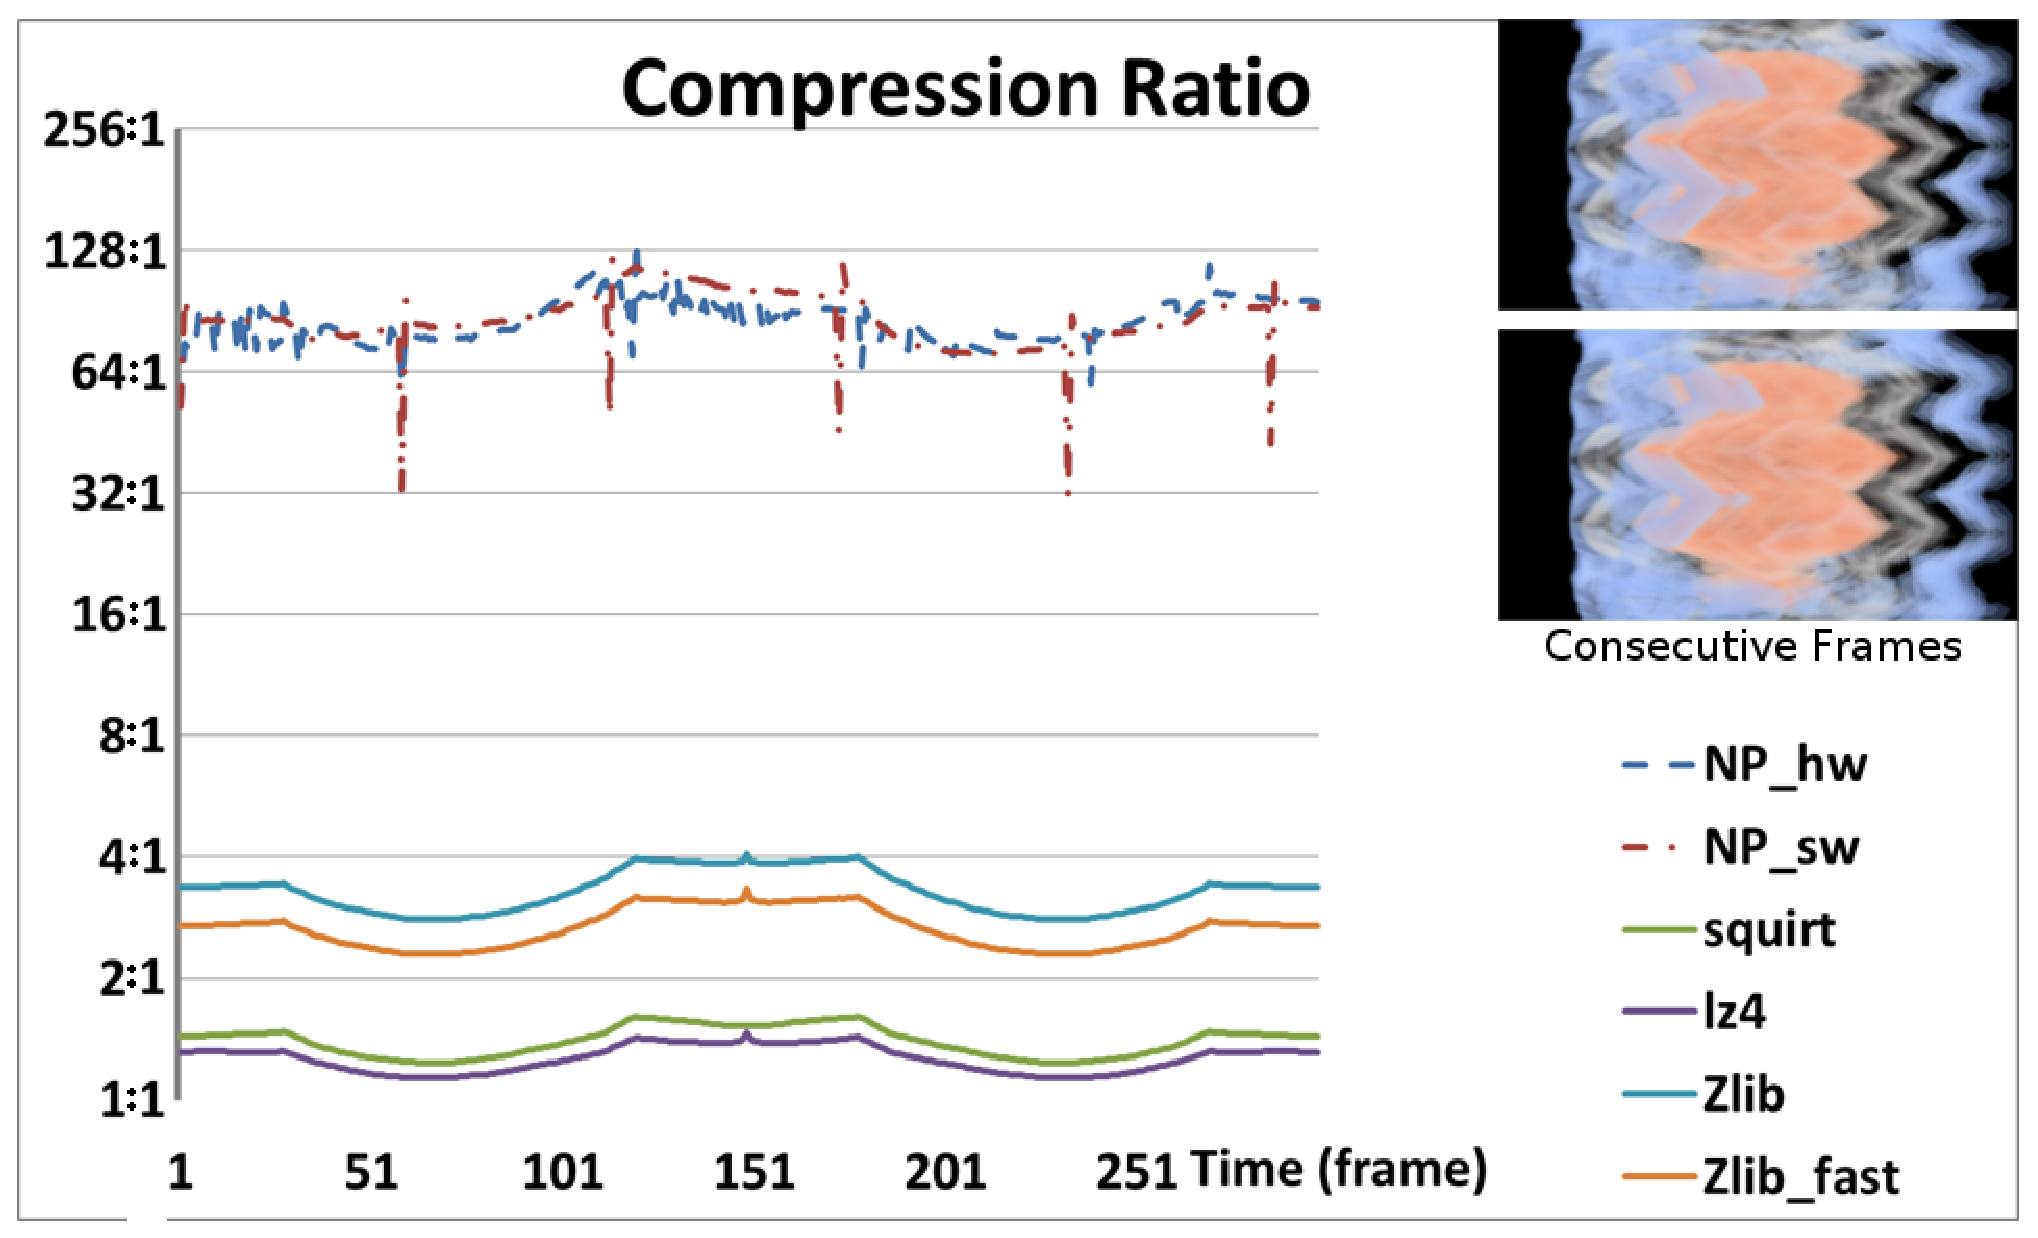
\includegraphics[width=\columnwidth]{compressRatio.eps}
  \caption{Compression ratio for `high coherency' case.
	H.264 achieves compression ratios above 128:1 whereas ParaView's existing
	compressors maxed out at 3.4:1 in our experiments.}
%  a large compression ratio advantage with above 128:1 versus ParaView's
%  compressors staying between 1.3:1 to 3.4:1.}
  \label{fig:compressRatio}
\end{figure}

~\cref{fig:compressRatio} shows per-frame compression ratios for
our `high coherency' configuration.  The occasional dips represent
when we send a keyframe, currently once every 60 frames.  Even if the
library were to use a keyframe for every frame, our library achieves
compression ratios 16x better than existing approaches.

% discuss the bandwidth reduction ( compare other paraview compressor )

~\cref{fig:time} shows the achievable frames/second for our
encoder as well as ParaView compressors.  Zlib is not competitive
for image compression.  While the best performance is achieved when
our library utilizes a GPU, lz4 and Squirt are competitive.  The
software-backed version of our library is slower than existing ParaView
solutions, so environments without a GPU will need to choose between
fast compression/decompression or low bandwidth.

The average compression ratio \(r_c\) is shown
in~\cref{tab:latency}.  Our library achieves a 42x better
compression rate than its closest competitor, Zlib.  The payload size
is particularly important in visualization because of the synchronous
nature of current tools: with only a frame or two of latency, it is
difficult to fully utilize network bandwidth.

%The theoretical aggregated latency could be calculated
%through Equation~\cref{eq:latency}, where communication time
%\(t_{network}=\frac{\text{compressed image size}}{BW}\).
%
%\begin{equation}
%\label{eq:latency}
%T_{latency}=t_{compression}+t_{decompression}+t_{network}
%\end{equation}
%
%Assume we have 10mbps available bandwidth, with average compressed
%image size \(\frac{1920*1080*8*3}{r_c}\) we could calculate
%the communication time for each compressor. Combining data
%from~\cref{fig:time} we get the overall latency in~\cref{tab:latency}.

% discuss encoding/decoding time --> framerate / latency 
\begin{figure}[t]
  \centering
  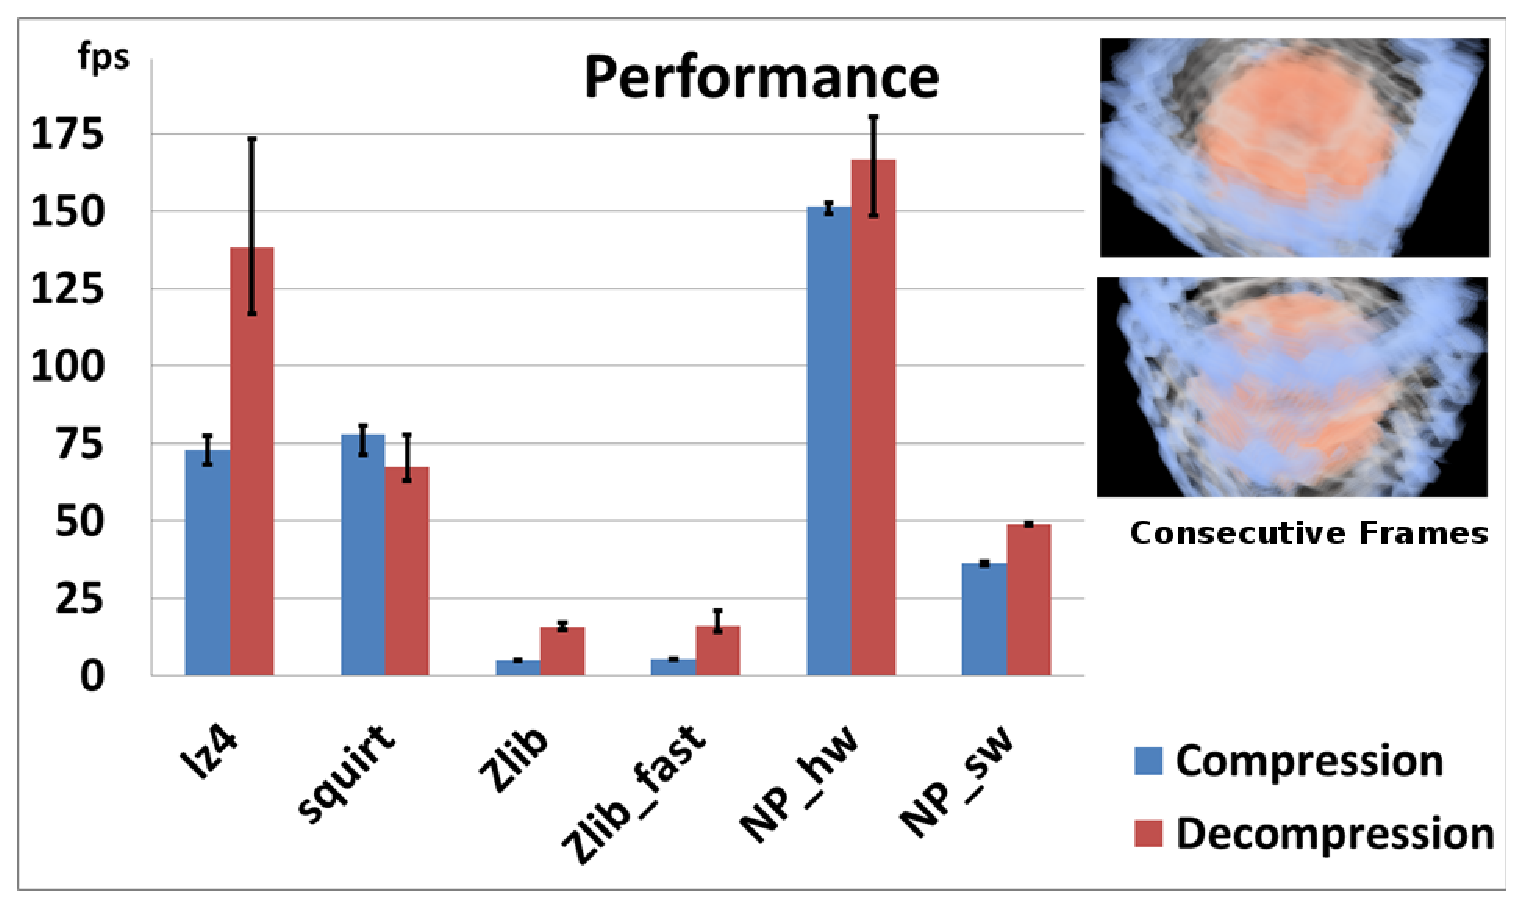
\includegraphics[width=\columnwidth]{Performance.eps}
  \caption{Frame rate of compression and decompression in our `low
  coherency' experiments.  Our libary's hardware-based backend achieves
  slightly better performance than competors, while delivering far
  smaller payloads.}
  \label{fig:time}
\end{figure}

\begin{table}[htb]
  \caption{Compression ratio in `low coherency' experiments. Our library has 42x
   better space saving than the closest compressor, Zlib.}
  \label{tab:latency}
  \scriptsize
  \begin{center}
    \begin{tabular}{ccccccc}
      & LZ4 & Squirt & Zlib & Zlib\_fast & NP\_hw & NP\_sw \\
    \hline
      \(r_c\) & 1.29:1 & 1.43:1 & 3.43:1 & 2.78:1 & 144:1 & 152:1 \\
    \end{tabular}
  \end{center}
\end{table}


\section{Conclusion}

%NvPipe exhibits competitive efficiency among other compressors in
%\cref{fig:time}. The average overall compression and decompression time
%is only 12.78ms. And the average encoding and decoding time for FFmpeg
%API call are 3.938ms and 3.029ms. They yield framerates of 254fps and
%330fps respectively. Because of the overhead introduced through FFmpeg
%wrapper they are expected to be lower than 398fps/658fps released by
%\cite{ref_1}.% cite nv codec menu.

Our library is an improvement upon existing visualization systems'
remote image delivery mechanism.  It saves greater than 42x bandwidth
in most cases, with modest improvements to compression/decompression
time as well.  While we utilize lossy H.264 at present, the induced
artifacts are minor.

% This is Peter's add-on for conclusion.

For future work, we would like to investigate the use of H.264's
lossles configuration~\cite{sullivan2012overview}.  With ParaView's
decomposition of `interactive' versus `still' renders, one could
envision using the lossy system during interaction with lossless
mode during pauses.  We would also like to investigate adding more
asynchronicity in the compression process: the synchronous nature of
visualization systems such as ParaView and VisIt makes it difficult
to fill a network pipe.  This is exacerbated by the high compression
ratios that are achieved with H.264.  Furthermore, since the encoding
hardware is asynchronous with the rest of the GPU, it should be
possible to completely hide the entire multi-millisecond encoding
latency.  Finally, as rendering already uses the GPU, we would like to
source the input images directly from the GPU buffer to avoid copying
images over PCIe in uncompressed form.

%In future research it will be intereting to investigate the performance
%of lossless H.264 configuration and HEVC
%standard~\cite{sullivan2012overview} provided with NVIDIA NvENC
%API. Other areas of investigations are towards more asynchronocity in
%this compression process: NvENC is entirely asynchronous to the rest of
%the GPU, with the potential to completely hide the encoding latency. On
%the other hand, software only approaches will not be able to fully hide
%that cost.

%\acknowledgements{
%NVIDIA standard acknowledgement for funding?
%}

%\pagebreak

\bibliographystyle{abbrv}
%%use following if all content of bibtex file should be shown
%\nocite{*}
\bibliography{template}
\end{document}
